\documentclass[11pt,letterpaper]{article}
\usepackage[lmargin=1in,rmargin=1in,tmargin=1in,bmargin=1in]{geometry}
\usepackage{../style/homework}
\usepackage{../style/commands}
\setbool{quotetype}{true} % True: Side; False: Under
\setbool{hideans}{true} % Student: True; Instructor: False

% -------------------
% Content
% -------------------
\begin{document}

\homework{3: Due 09/18}{Fire can't go through doors, stupid. It's not a ghost.}{Ben Chang, Community}

% Problem 1
\problem{10} Consider the triangle given below:
	\[
	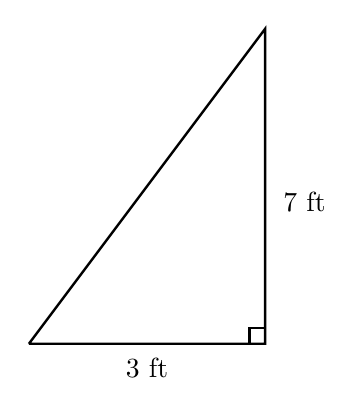
\begin{tikzpicture}
	\draw[line width=0.03cm] (0,0) -- (3,0) -- (3,4) -- (0,0);
	\draw[line width=0.03cm] (2.8,0) -- (2.8,0.2) -- (3,0.2);
	\node at (1.5,-0.3) {$3$~ft};
	\node at (3.5,1.8) {$7$~ft};
	\end{tikzpicture}
	\]

\begin{enumerate}[(a)]
\item Find the perimeter of the triangle.
\item Find the area of the triangle. 
\item If the lengths of the legs in the triangle were mislabeled as being in feet when they should have been in meters, convert your answer in (b) to square meters. 
\end{enumerate}



\newpage



% Problem 2
\problem{10} Consider the `track' shown below:
	\[
	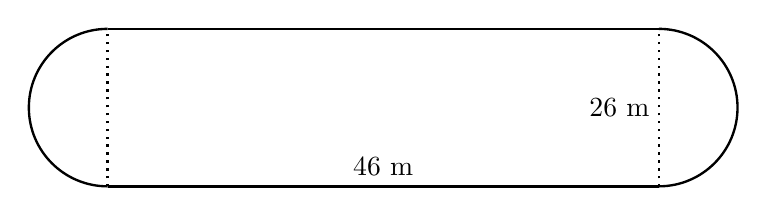
\begin{tikzpicture}
	\draw[line width=0.03cm] (0,0) -- (7,0);
	\draw[line width=0.03cm] (0,2) -- (7,2);
	
	\draw[line width=0.03cm,dotted] (0,0) -- (0,2);
	\draw[line width=0.03cm,dotted] (7,0) -- (7,2);
	 
	\draw[line width=0.03cm] (0,2) arc(90:270:1);
	\draw[line width=0.03cm] (7,0) arc(270:450:1);
	
	\node at (3.5,0.25) {$46$~m};
	\node at (6.5,1) {$26$~m};
	\end{tikzpicture}
	\]

\begin{enumerate}[(a)]
\item Find the perimeter of the track.
\item Find the area of the track.
\item If you scale the track's size by a factor of two, what is the new perimeter and area?
\item Suppose you were going to tile the interior rectangular portion of the track with special 2~m $\times$ 2~m tiles. How many would you need?
\end{enumerate}



\newpage



% Problem 3
\problem{10} A whiskey barrel is approximately cylindrical in shape. Suppose that an American Oak whiskey barrel is 18~in across and 30~in tall.
	\begin{enumerate}[(a)]
	\item Estimate the volume of the barrel. 
	\item If one cubic inch is 16.3871~ml, find the volume of the barrel in milliliters. 
	\item You know expensive whiskeys can fetch \$450 per bottle, i.e. 750~ml. Use this to estimate the value of such a barrel filled with expensive whiskey if the barrel itself also has a value of \$250.
	\end{enumerate}


\end{document}